\chapter{Mathematical Considerations}
\label{ch:math}

\section{Zipf's laws in RecSys and the Matthew Effect}

In a great many applications of machine learning, a caveat is given early, that the distribution of observations of unique items from a large corpus is modeled by Zipf's law. In recommendation systems, the \emph{Matthew Effect} appears in the popular item's click rates, or the popular user's feedback rates. 

Simply, the Matthew Effect–or popularity bias–states that the most popular items continue to attract the most attention and widen the gap with other items. Take for example the MovieLens dataset, an extremely popular dataset for benchmarking recommendation systems[link to MovieLens info], in [[Jenny Sheng 2020]\url{https://jennysheng.com/jenny-sheng-iw-fall-2020.pdf}] they observe the following behavior for number of movie ratings:

\vspace{10pt}
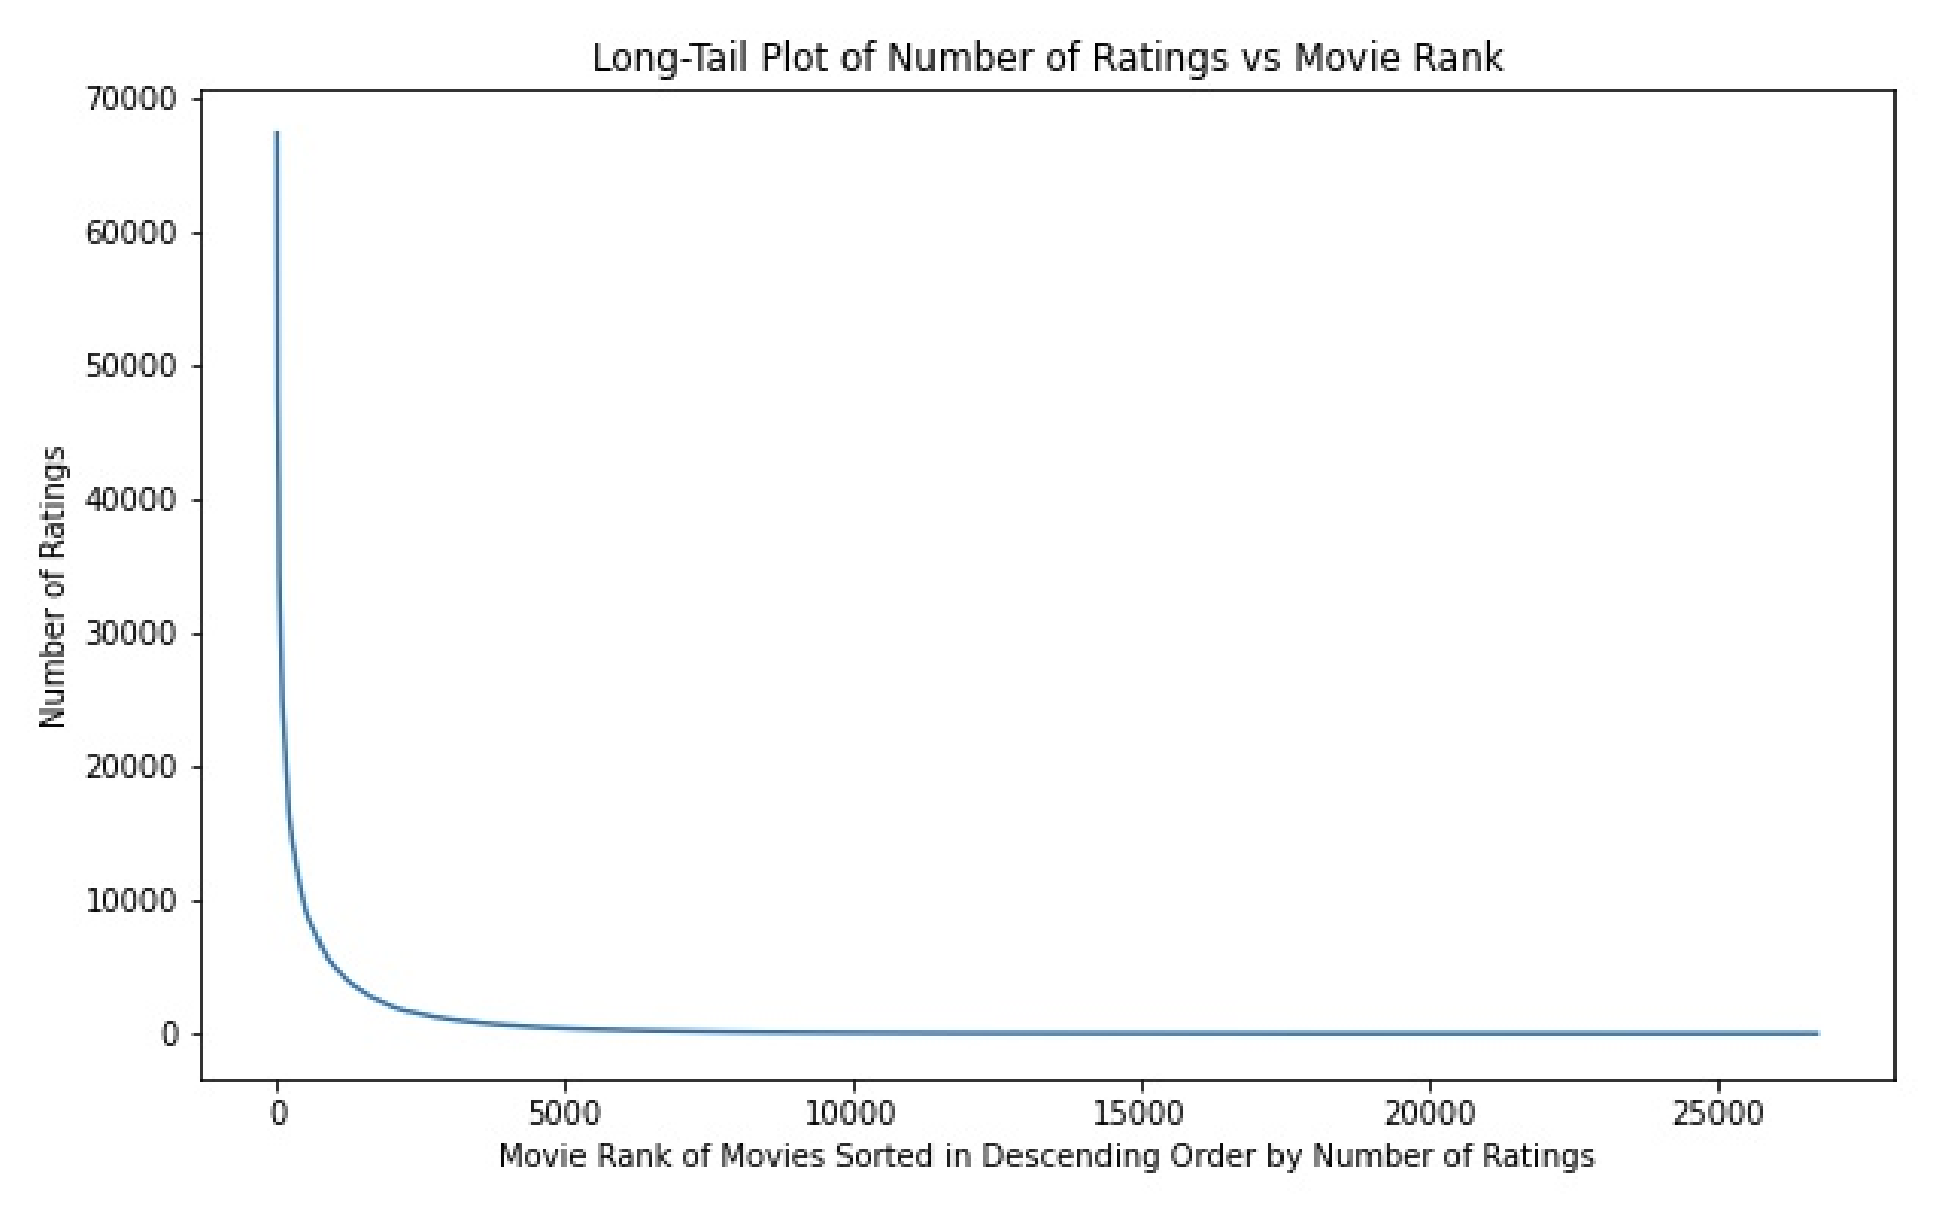
\includegraphics[width=\textwidth-10pt]{book-text/zipfian-moverank.png}

At first glance this behavior is obvious and stark, but is it a problem? Let's assume our recommender will be built as a user-based CF model–as alluded to in \ref{ch:user-item}–then how might these distributions effect the recommender?

Let the probability mass function be described by the simple Zipf's law:

\begin{equation}
    f(k, M) = \frac{1/k}{\sum^M_{n=1}(1/n)}    
\end{equation}


for $M$ number of tokens in the corpus (in the above examples number of movies), $k$ is the rank of a token when sorted by number of occurrences. 

Let's consider users $A$ and $B$, with $N_A = \mathcal{I}_A$  and $N_B = \mathcal{I}_B$ ratings respectively, Observe that the probability of $V_i$, the $i$'th most popular video, appearing in $\mathcal{I}_X$ for some user $X$ is given by:
\begin{equation}
    P(i)=\frac{f(i,M)}{\sum^M_{j=1}f(j,M)}=\frac{1/i}{\sum^M_{j=1}1/j}
\end{equation}

and thus the joint probability of an item appearing in two user's ratings is:

\begin{equation}
  P(i^2)=\left(\frac{1/i}{\sum^M_{j=1}1/j}\right)^2.  
\end{equation}

This becomes important when one also considers that our, yet unstated, definition of user-based collaborative filtering, is based on similarity in user's ratings sets–**number of jointly rated items by two users, divided by the total number of items rated by either.**

Taking this definition, we can for example, compute the similarity score for one shared item amongst $A$ and $B$:

\begin{equation}
    \sum^M_{i=1} \frac{P(i^2)}{\| \mathcal{I}_A \cup \mathcal{I}_B \|},
\end{equation}

and the average similarity score of two users is generalized to:

\begin{equation}
    \sum^{\min(N_A,N_B)}_{t=1}\left(\prod_{i_k=i_{k-1}+1}^{t-1}\sum^M_{i=1} \frac{P({i_k}^2)}{\frac{\| \mathcal{I}_A \cup \mathcal{I}_B \|}{t}}\right).
\end{equation}

These combinatorial formulas indicate not only the relevance of the Zipfian in our algorithms, but we see an almost direct effect on the output of scores. Consider the experiment from [(Wang, Wang, and Zhang 2019)]\url{https://arxiv.org/abs/1909.12798}; for LastFM users, the authors demonstrate average similarity scores for pairs of users, and they find this Matthew Effect persists into the similarity matrix:

\vspace{10pt}
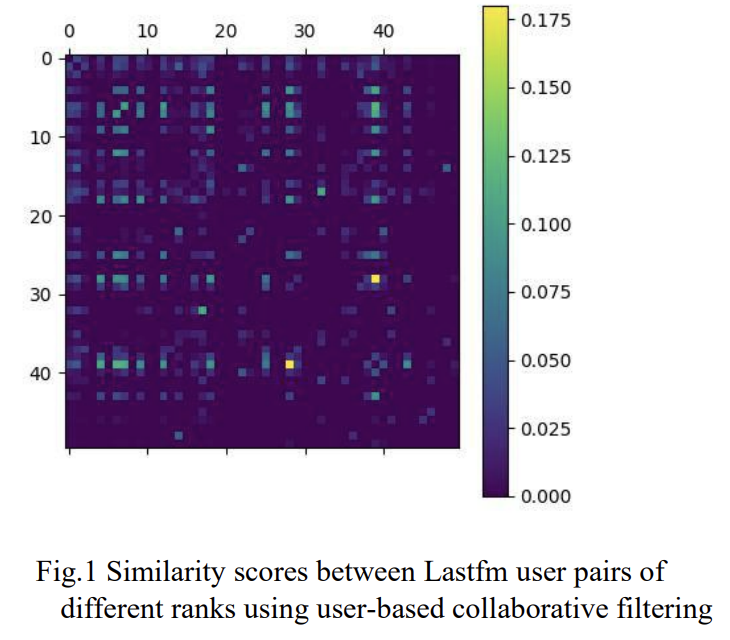
\includegraphics[width=\textwidth-10pt]{book-text/lastfm-matthew-effect.png}

While these results might seem scary, we'll observe later via diversity-aware loss functions that we can mitigate some of this. An even simpler way, is to use downstream sampling methods, which we will discuss as part of our explore-exploit algorithms. Finally, the Matthew Effect is only the first of two major impacts of this Zipfian–let's turn our attention to the second.